% !TEX program = xelatex

\documentclass[hidelinks, 12pt, a4paper]{article}

\usepackage{fontspec}
\setmainfont[Ligatures=TeX]{Linux Libertine O}

\usepackage[hidelinks, colorlinks = true, urlcolor = blue]{hyperref}

\usepackage{indentfirst}
\usepackage{graphicx}
\usepackage[left=2cm,right=2cm,top=2cm,bottom=2cm]{geometry}
\usepackage{lipsum}
\usepackage{caption}
\usepackage{subcaption}
\usepackage{dirtytalk}
\usepackage[autostyle]{csquotes}
\usepackage{epigraph}


\begin{document}
\sloppy % this is legendary

\begin{titlepage}

\begin{figure}[h!]
  \begin{center}
    
\includegraphics[width=3cm]{assets/auth.pdf}
    \label{fig:cover_auth_logo}
  \end{center}
\end{figure}

\centering
\Large Αριστοτέλειο Πανεπιστήμιο Θεσσαλονίκης\\
\Large Πολυτεχνική Σχολή\\
%\large Τμήμα Ηλεκτρολόγων Μηχανικών και Μηχανικών Υπολογιστών\\
%\large Τομέας Τηλεπικοινωνιών

\vspace{\fill}

\LARGE \textbf{Java socket programming} \\
\LARGE \textbf{Δίκτυα 2}

\vspace{\fill}

\Large Θεόδωρος Κατζάλης \\
\Large ΑΕΜ:9282 \\ 
\Large katzalis@auth.gr

\vspace{\fill}
\raggedright

\centering
\vspace{\fill}
\today

\end{titlepage}

%\maketitle


\pagebreak
\tableofcontents
\pagebreak

% \section{Lorem}
% \lipsum


\section{Εισαγωγή}

Η συγκεκριμένη εργασία αποσκοπεί στην εξοικείωση εννοιών σχετικά με τα δίκτυα υπολογιστών τόσο σε θεωρητικό όσο και σε πρακτικό επίπεδο. Αυτό εξασφαλίζεται με την δημιουργία δικτυακών εφαρμογών χρησιμοποιώντας την γλώσσα προγραμματισμού \textbf{java} σε συνεργασία με τον server ithaki του μαθήματος με IP 155.207.18.208. Αυτή λοιπόν η συνεργασία επιτρέπει \textbf{active} έλεγχο και καθορισμό ορισμένων παραμέτρων αλλά και \textbf{passive} συλλογή δεδομένων επειτα απο συγκεκριμένα request του χρήστη στον server. Προς το τέλος αυτού του report θα γίνει αναφορά για πρωτόκολλα UDP και audio streaming.

Ενδεικτικά θα σημειώσουμε τις εφαρμογές που βασιστήκαμε για να συλλέξουμε πληροφορίες απο την πλευρά του client με μια σύντομη περιγραφή τους. Η πλειοψηφία αυτών βασίζεται στο πρωτόκολλο UDP. 
\begin{itemize}
    \item \textbf{Echo}.
        Αποστολή μηνύματος της μορφής ΕΧΧΧX και λήψη πακέτου με δεδομένα που αφορούν την τρέχουσα ημερομηνία και ώρα.
    \item \textbf{Image}.
        Αποστολή μηνύματος της μορφής ΜΧΧΧΧ και λήψη πακέτων που περιλαμβάνουν το byte content μιας φωτογραφίας jpg. The challenge: Βρες τους delimiters, την αρχή και το τέλος της εικόνας 
    \item \textbf{Audio}.
        Αποστολή μηνύματος της μορφής ΑΧΧΧΧ και λήψη πακέτων ήχου κωδικοποιημένα σε DPCM και AQ-DPCM. The challenge: Κατανόηση της κωδικοποίησης/αποκωδικοποίησης και βελτίωση της ποιότητας του ήχου.
    \item \textbf{Ithakicopter}. Συλλογή τηλεμετρίας απο custom κατασκευή προσομοίωσης ελικοπτέρου. The challenge: Autopilot
    \item \textbf{Car vehicle diagnostics}. Συλλογή διαγνωστικών στοιχείων απο μια βάση δεδομένων σχετικά με κάποια στοιχεία λειτουργίας ενός αυτοκινήτου. The challenge: Υλοποίηση υπολογισμού δεδομένων και εισαγωγή στο πρωτόκολλο TCP και τα streams.
\end{itemize}


Όσον αφορά τα διαγράμματα που χρησιμοποιήθηκαν στα session1.pdf και session2.pdf, για λόγους πληρότητας, θα αναφέρουμε ότι τα ιστογράμματα έγιναν με την χρήση του λογισμικού στατιστικής SPSS και όλα τα υπόλοιπα με την χρήση της βιβλιοθήκης matplotlib της γλώσσας προγραμματισμού python! Επίσης όλα τα αρχεία γράφτηκαν σε \LaTeX και το εξώφυλλο είναι ένα Overleaf template, το οποίο μπορείτε να βρείτε \href{ https://www.overleaf.com/latex/templates/protupo-diplomatikis-ergasias-thmmy-apth/kdffpgptgbzc}{εδώ}.

\subsection{Statement of originality}

\epigraph{"Let the work speak for itself..."}

Στα πλαίσια του \textbf{statement of originality}, ελπίζουμε τα logs\footnote{Η cosmote άλλαξε πρόσφατα την public IP. Η κύρια IP η οποία φαινόταν προγενέστερα ήταν 87.202.99.165 (router.pdf)} της ιθάκης, το report, τα διαγράμματα και ο κώδικας να μιλήσουν απο μονά τους. Στο τέλος, έχουμε παραθέσει βιβλιογραφία για τις πηγές στις οποίες βασιστήκαμε για να φέρουμε εις πέρας αυτήν την εργασία. Στο κομμάτι του κώδικα, αρχικός κόμβος ερεθισμάτων αποτέλεσε η αναφορά του ίδιου του μαθήματος, οπότε θα την παραθέσουμε και πρώτη\cite{ergasia2}. Οι διαλέξεις και οι διαφάνειες βοήθησαν επίσης σε μεγάλο βαθμό για την κατανόηση βασικών εννοιών (NAT translation, OSI stack, client-server architecture).

\pagebreak
\section{Session 1}


Σχετικά με την χρονοκαθυστέρηση και την ρυθμαπόδοση των echo packets έχουμε να αναφέρουμε τα εξής:

\subsection{Echo packets Delay: ON}

\subsubsection{Χρόνος απόκρισης}
\begin{itemize}
    \item Μέση τιμή: 1815 milliseconds και τυπική απόκλιση: 557 milliseconds
    \item Αρκετά υψηλή η δεύτερη σε σύγκριση με την πρώτη το οποίο υποδηλώνει ότι τα δείγματα μεταξύ τους δεν είναι "συμπυκνωμένα"και αποκλίνουν σημαντικό βαθμό απο την μέση τιμή.
    \item Δεν φαίνεται με ξεκάθαρο τρόπο ποια κατανομή ακολουθούν τα δεδομένα μας, ωστόσο με κάποια επιφύλαξη θα μπορούσαμε να ισχυριστούμε ότι ακολουθούν bimodal κατανομή. Αυτό το συμπέρασμα προέκυψε απο την τάση να σχηματιστούν δύο καμπάνες.
\end{itemize}

\subsubsection{Ρυθμαπόδοση}

\begin{itemize}
    \item Μέση τιμή: 109 bits/sec και τυπική απόκλιση: 30.04 bits/sec
    \item Ομοίως με την μελέτη της χρονικής απόκρισης, η τυπική απόκλιση είναι αρκετά υψηλή, περίπου το 30\% της μέσης τιμής.
    \item Σχετικά με την κατανομή, θα μπορούσαμε να υποστηρίξουμε ότι είναι μια right skew κατανομή μιας και παρουσιάζει μια ασυμμετρία γύρω απο την μέγιστη τιμή.
\end{itemize}
Παρατηρώντας το διάγραμμα της \textbf{ρυθμαπόδοσης} (throughput) διακρίνουμε ότι το εύρος τιμών κυμαίνεται περίπου απο 70 μέχρι 180 bits/second. Αξίζει να σημειωθούν κάποιες σχεδιαστικές αποφάσεις οι οποίες λήφθηκαν κατα τη διάρκεια υλοποίησης του αλγορίθμου της ρυθμαπόδοσης:

Σύμφωνα με την περιγραφή της άσκησης, ο υπολογισμός έπρεπε να γίνει με την \textbf{τεχνική του κινούμενου μέσου όρου}. Επιλέξαμε τα 8 δευτερόλεπτα ως το χρονικό πλαίσιο λήψης δεδομένων για κάθε δείγμα ρυθμαπόδοσης το οποίο υπολογίζεται για κάθε δευτερόλεπτο σε μήκος 4 συνεχόμενων λεπτών λήψης echo packets. Συνεπώς για τα τελευταία 8 δευτερόλεπτα απο τα 4 λεπτά της συνολικής μέτρησης δεν έχουν υπολογιστεί δείγματα ρυθμαπόδοσης. 

Η ύπαρξη των \textbf{spikes} στο διάγραμμα ερμηνεύεται απο το αν πρόλαβε κάποιο πακέτο στο πλαίσιο των 8 δευτερολέπτων να συμπεριληφθεί στο ένα δείγμα και όχι στο άλλο. Για παράδειγμα, αν έρθει ένα πακέτο την χρονική στιγμή $t_1 = t + 6.5$ second, και το επόμενο έρθει την χρονική στιγμή $t_2 = t + 8.1$, τότε το δείγμα της ρυθμαπόδοσης που μετρούσε στο εύρος $[t, t+8]$ δεν θα λάβει υπόψιν το πακέτο που έφτασε στα $t + 8.1$. Ωστόσο στο δείγμα της ρυθμαπόδοσης με εύρος μέτρησης $[t+8, t+16]$ θα συμπεριληφθεί η τιμή του. Συγκεκριμένα, η τιμή αυτή είναι $32*8$ bits, αφού το κάθε echo packet response περιέχει 32 bytes\footnote{Ο τρόπος με τον οποίο διαπιστώσαμε το μέγεθος των δεδομένων έγινε με την βοήθεια του wireshark} δεδομένα. Για αυτό μπορούμε να παρατηρήσουμε ότι τα spikes διαφέρουν απο τα υπόλοιπα δείγματα πολλαπλάσια του $32$. Σε μια zoom out έκδοση του γραφήματος θα φαινόταν σίγουρα μια πιο ομαλή καμπύλη.


\subsection{Echo packets Delay: OFF}

\subsubsection{Χρόνος απόκρισης}
Στην συγκεκριμένη περίπτωση η χρονοκαθυστέρηση των δειγμάτων μειώνεται αισθητά σε χαμηλότερες τιμές milliseconds με αποτέλεσμα να λαμβάνουμε αρκετά περισσότερα δείγματα συγκριτικά με την προηγούμενη περίπτωση. Συνεπώς για λόγους ευκρίνειας\footnote{engineering appreciation όπως έχει ειπωθεί και στο μάθημα} παραθέτουμε μια zoom in εκδοχή του διαγράμματος του χρόνου απόκρισης με εύρος ενδεικτικά 100-200 packets. Σε γενικές γραμμές το εύρος της χρονοκαθυστέρησης κυμαίνεται απο 230-260 milliseconds. Πιο συγκεκριμένα έχουμε:
\begin{itemize}
    \item Μέση τιμή: 237 milliseconds και τυπική απόκλιση: 7 milliseconds 
    \item Συγκριτικά με Delay: ON, βλέπουμε ότι η τυπική απόκλιση είναι αρκετά μικρή σε σχέση με την μέση τιμή, επομένως τα δείγματα δεν έχουν την τάση να είναι "αραιωμένα".
    \item Σχετικά με την κατανομή, μπορούμε να διακρίνουμε την δημιουργία δύο στενών καμπανών γύρω απο τις τιμές 232 και 246. Συνεπώς θα μπορούσαμε να ισχυριστούμε για μια ακόμη φορά bimodal distribution. 
\end{itemize}

\subsubsection{Ρυθμαπόδοση}
Για τις σχεδιαστικές αποφάσεις καθώς και την ερμηνεία των spikes, έχει γίνει ήδη αναφορά στην προηγούμενη ανάλυση (Delay: ON).

Όπως έχει αναφερθεί, ο αριθμός των πακέτων που φτάνουν στον δέκτη είναι πολύ μεγαλύτερος με μικρότερη χρονοκαθυστέρηση μεταξύ των πακέτων, συνεπώς η ρυθμαπόδοση αυξάνεται αισθητά.
\begin{itemize}
    \item Μέση τιμή: 1040 bits/sec και τυπική απόκλιση: 18 bits/sec.
    \item Εξίσου μικρή η τυπική απόκλιση συγκριτικά με την μέση τιμή.
    \item Σχετικά με τη κατανομή, μιας και οι τιμές συγκεντρώνεται στο αριστερό κομμάτι του γραφήματος, θα μπορούσαμε να υποθέσουμε λογαριθμική.
\end{itemize}


'Οσα έχουν αναφερθεί μέχρι στιγμής αφορούν τον σχολιασμό των διαγραμμάτων G1-G8.

\subsection{Retransmission timeout (RTO)}


Για λόγους γρήγορης και αξιόπιστης επικοινωνίας σχετικά με το πρωτόκολλο TCP, υπάρχει η ανάγκη πρόβλεψης και επαναπροσδιόρισης των παραμέτρων timeout σε ένα σύστημα επικοινωνίας. Πόσο πρέπει να περιμένει ο sender αν δεν λάβει  ACK απο τον receiver για να ξαναστείλει την πληροφορία; Ο προσδιορισμός των timers είναι λοιπόν πολύ σημαντικός διότι αν δεν ρυθμιστεί σωστά, υπάρχει η πιθανότητα να ξανασταλθεί πακέτο πολύ γρήγορα προτού ο δέκτης να προλάβει να στείλει ACΚ ή το ανάποδο, δηλαδή να περιμένει πολύ να ξαναστείλει ένα πακέτο\cite{gfg_rto, saminir}. 

Υπάρχουν κάποιες μαθηματικές σχέσεις οι οποίες υπολογίζουν τον retransmssion timer και υπάρχουν συγκεκριμένα 3 σταθερές \textbf{α, β και γ}. Εμείς επιλέξαμε αρχικά σταθερά τα α και β με τιμές $1 - 1/8 = 0.875$ και $1 - 1/4 = 0.750$. Εσκεμμένα γράψαμε με αυτήν την μορφή τις εξισώσεις προκειμένου να είμαστε συμβατοί με το notation των εξισώσεων που μας δίνονται στα πλαίσια του μαθήματος, μιας και οι αναφορές\cite{rfc}, τα δικά μας α και β, τα συμβολίζουν ως (1-α) και (1-β). Για την επιλογή του γ (k σύμφωνα με RFC) δοκιμάσαμε στην αρχή την προτεινόμενη τιμή 4. Στη συνέχεια παρατηρώντας το γράφημα R1 προσπαθούσαμε να φτάσουμε την γραμμή RTO να αγκαλιάζει το RTT, δηλαδή να μην είναι πολύ πάνω αλλά και ούτε απο κάτω του RTT. Τελικά επιλέξαμε την τιμή 1,8 και βλέπουμε ότι ικανοποιητικά η γραμμή RTO ακολουθεί σωστά το RTT.



\subsection{Image}

Κατά τη διάρκεια ανάπτυξης της εφαρμογής της εικόνας. στην προσπάθεια μας να δημιουργήσουμε real-time video, αλλάξαμε το μέγεθος των πακέτων απο 128 σε 1024 bytes χρησιμοποιώντας το κατάλληλο request code. Καταφέραμε λαμβάνοντας 100 δείγματα να δημιουργήσουμε ένα βίντεο 40 δευτερολέπτων κάνοντας merge τα δείγματα αυτά. Το video μπορείτε να το δείτε \href{https://drive.google.com/file/d/1yfwckvGBr8YteigF3ainMJMXwLOzjZ9u/view?usp=sharing}{εδώ}. Αξίζει να σημειωθεί οτι για το βίντεο χρησιμοποιήσαμε την κάμερα FIX. Θα μπορούσαμε να χρησιμοποιούσαμε την PTZ για να είχαμε πιο πιστευτή πραγματική αναπαράσταση μιας και ο χρόνος λήψης της εικόνας είναι πιο μικρός εξαιτίας της μικρότερης ανάλυσης της.

Σχετικά με τον χρόνο που αποτυπώνουν οι εικόνες, παρατηρήσαμε οτι στην FIX η ημερομηνία και η ώρα είναι ακριβής, ενώ στην PTZ υπάρχει μια καθυστέρηση της τάξης των 4 λεπτών περίπου. Φυσικά με κατάλληλες εντολές DIR=X, υπάρχει και η δυνατότητα απεικόνισης του πύργου του ΟΤΕ (session 2)!

Σχετικά με την υλοποίηση  της λήψης της εικόνας, ελέγχουμε σε κάθε πακέτο που λαμβάνουμε αν υπάρχει ο delimiter \textbf{OxFF D9}. Αυτή η πληροφορία θα σηματοδοτούσε το τέλος της εικόνας και έπειτα γράφοντας τα δεδομένα σε ένα αρχείο jpg, υπάρχει η δυνατότητα προβολής. Ωστόσο, αξίζει να αναφέρουμε ότι εξαιτίας ενδεχομένως θορύβου κβάντισης και καναλιού, αυτός ο delimiter μπορεί να μην εντοπιστεί. Βέβαια σε πρώιμες υλοποιήσεις, στις οποίες δεν ελέγχαμε αν υπήρχαν delimiters, αποθηκεύαμε όλη την πληροφορία και υπήρχε εξίσου η δυνατότητα προβολής (ακόμα και αν υπήρχαν περισσότερα bytes στο τέλος της εικόνας μετά τον delimiter OxFF D9). Μιας και δεν ειπώθηκε κάτι για τα bytes που σηματοδοτούν την έναρξη της εικόνας, παρατηρήσαμε απο το wireshark ότι η πρώτη πληροφορία που λαμβάνουμε είναι το OxFF D8 (start of image).

\subsection{Audio}

Σχετικά με τον ήχο χρησιμοποιήσαμε τους κωδικούς L11 (second clip AQ-DPCM) και L22  για τα ζητούμενα της εργασίας: 
\begin{itemize}
    \item L11: René Aubry\footnote{Τρομερός συνθέτης. Τυχερός που τον βρήκα στο L11.}, Après la pluie II
    \item L22: Edward Maya \& Vika Jigulina, Stereo Love
\end{itemize}

Όσον αφορά τα γραφήματα του ήχου μπορούμε να παρατηρήσουμε το λεγόμενο \textbf{clipping effect}. Εξαιτίας της αναδρομικής σχέσης στην αποκωδικοποίηση DPCM και AQ-DPCM για την λήψη των πραγματικών δειγμάτων, υπάρχει περίπτωση οι τιμές των samples να υπερβούν τις μέγιστες και τις ελάχιστες των 8 και 16 bits προσημασμένου ακεραίου που χρησιμοποιήθηκαν για την κβάντιση τους. Οπότε προκειμένου να αποφύγουμε το ενδεχόμενο να γίνει roll back απο την μεγαλύτερη τιμή στην μικρότερη, κάθε φορά που ο integer (32 bits) ξεπερνούσε την μέγιστη τιμή ή την ελάχιστη τιμή των bits κωδικοποίησης, τότε το θέταμε ίσο με το μέγιστο ή το ελάχιστο αντίστοιχα. Για αυτό το λόγο επίσης μπορούσε να ερμηνεύσουμε και στο ιστόγραμμα, ιδιαίτερα υψηλές τιμές στις ελάχιστες όπου γινόταν το clipping.

Επειδή ο αριθμός των δειγμάτων είναι ιδιαίτερα υψηλός, έχουμε προσθέσει στα διαγράμματα ήχου και zoom in εκδοχές προκειμένου να έχουμε μια αίσθηση του τρόπου διακύμανσης των τιμών σε τοπικό επίπεδο. Ενδιαφέρον παρουσιάζει το διάγραμμα του τόνου, απο την εικονική γεννήτρια συχνοτήτων, στο οποίο μπορούμε να παρατηρήσουμε το σχηματισμό ενός ημιτονοειδούς/τριγωνικού σήματος!

Σχετικά με την μέση τιμή, η οποία προστίθεται στα δείγματα, έχει μικρή τιμή συγκριτικά με τις διαφορές των δειγμάτων οι οποίες καθορίζονται σε μεγάλο βαθμό απο τις μεγάλες τιμές του step.

Το request code audio που φαίνεται στο wireshark αντιστοιχίζεται στην κυματομορφή AQ-DPCM (G9), ενώ τα υπόλοιπα δείγματα έχουν ληφθεί για το ίδιο τραγούδι αλλά διαφορετικές χρονικές στιγμές.

\subsubsection{AQ-DPCM}

\begin{itemize}
    \item Το ιστόγραμμα των διαφορών των δειγμάτων για AQ-DPCM δείχνει μια τριγωνική/κανονική κατανομή αν και παρουσιάζεται μια έντονη ασυμμετρία γύρω απο ένα spike. Αυτό εμφανίζεται στην τιμή 0, το οποίο σημαίνει ότι κάποια δείγματα ήταν ίδια. Οι τιμές των δειγμάτων έχουν υψηλές τιμές της τάξης των χιλιάδων με μέση τιμή -48 και τυπική απόκλιση κοντά στα 4000.
    \item Το ιστόγραμμα των ίδιων των σημάτων φαίνεται να ακολουθεί μια κανονική κατανομή με μέση τιμή -11600 και τυπική απόκλιση 10282. Το clipping effect συμβάλει στο spike του ιστογράμματος, καθώς πολλές τιμές που υπερβαίνουν τα όρια συγκεντρώνονται σε εκείνη την περιοχή, δηλαδή την ελάχιστη τιμή των 16 bits προσημασμένου ακεραίου.
\end{itemize}


\subsubsection{DPCM}

Το DPCM απο την άλλη πλευρά μας δείχνει δύο πολύ καθαρά γραφήματα όσον αφορά τις διαφορές των δειγμάτων και των ίδιων των δειγμάτων. Τα δεδομένα και στις δύο περιπτώσεις φαίνεται να ακολουθούν τριγωνική κατανομή. Αξίζει να σημειωθεί οτι οι τιμές είναι αρκετά πιο χαμηλές σε σύγκριση με το AQ-DPCM, μιας και θεωρούμε ότι το step (η επίδραση του step (>0) στον ήχο ήταν η ένταση του) είναι ίσο με 1, σε αντίθεση με το AQ στο οποίο μας έρχεται ως πληροφορία το step και έχει και ιδιαίτερα υψηλές τιμές επηρεάζοντας σημαντικά τις διαφορές των δειγμάτων και ως συνεπακόλουθο και τα ίδια τα δείγματα.

\subsubsection{Tone frequency}

Γνωρίζουμε ότι η εικονική γεννήτρια συχνοτήτων παράγει δύο ημίτονα και στέλνει την πληροφορία με κωδικοποίηση DPCM. Χρησιμοποιώντας το εργαλείο audacity, προκειμένου να βρούμε τις συχνότητες, παρατηρώντας τα spikes του spectrum plot, μπορούμε να εικάσουμε επιλέγοντας τις υψηλότερες κορυφές, ότι οι συχνότητες των ημιτόνων είναι \textbf{421} και \textbf{343 Hz}.

\begin{figure}[h!]
\centering
	\includegraphics[height=.3\textheight, width=\textwidth]{assets/session1/spectrum.png}
    \caption{Frequency spectrum απο δείγμα της εικονικής γεννήτριας συχνοτήτων}
\end{figure}


\subsection{Ithakicopter - autopilot}

Σχετικά με το ithakicopter επιλέγοντας AUTOPILOT:ON, έχουμε την δυνατότητα να καθορίσουμε ένα flightlevel στο οποίο το copter προσπαθεί με σταθερό ρυθμό να φτάσει και να παραμείνει εκεί. Βλέποντας την καμπύλη του ALTITUDE στα γραφήματα φαίνεται η ανοδική πορεία, μια μικρή σταθεροποίηση και έπειτα η πτώση (πατώντας AUTOPILOT:OFF). 

Στην δεύτερη μας μέτρηση πειραματιστήκαμε λίγο παραπάνω και επιτηδευμένα στείλαμε προς τα κάτω το copter αφού είχαμε φτάσει στο επιθυμητό flightlevel, ωστόσο ο μηχανισμός autopilot έκανε σωστά την δουλεία του και προσπάθησε να το επαναφέρει.


\textbf{Ithakicopter αλλα TCP version}: Προσπαθήσαμε και εμείς με την δική μας σειρά αρχικά να στείλουμε εντολές μέσω TCP και κατ' επέκταση να προσπαθήσουμε να υλοποιήσουμε τον μηχανισμό autopilot. Κάτι το οποίο αξίζει να αναφερθεί είναι ότι την στιγμή δημιουργίας του TCP socket, χωρίς να υπάρξει κάποιο write(), η ithaki μας έστελνε κάτι σαν εισαγωγικό μήνυμα το οποίο μας έλεγε κάποιες πληροφορίες για το format της εντολής που πρέπει να σταλθεί προκειμένου να έχει απόκριση ο server. Οπότε αυτά τα bits θα έπρεπε πρώτα να γίνουν skip, πρώτου γίνει προσπάθεια λήψης τηλεμετρίας μετά απο εντολή write(). 

Στα πλαίσια λοιπόν του TCP ithakicopter, προσπαθήσαμε στη συνέχεια να υλοποιήσουμε τον \textbf{autopilot}. Στην αρχή ο τρόπος με τον οποίο δημιουργήσαμε τις συναρτήσεις και τον σχεδιασμό της εργασίας οδήγησε στο να υλοποιηθεί μια ρουτίνα TCP η οποία και άκουγε αλλά και έστελνε πακέτα. Προκειμένου όμως να έχουμε μια ρουτίνα η οποία μόνο θα ακούει και ανάλογα το feedback θα πρέπει να στέλνει νέα commands, αποφασίσαμε να χρησιμοποιήσουμε ήδη το  UDP passive κομμάτι τηλεμετρίας και το TCP μόνο όταν πρέπει να στείλουμε νέες τιμές στα moters για να ελέγχουμε το ύψος. Προς το παρόν δεν έχει γίνει κάποιος μαθηματικός υπολογισμός (θεωρία Συστημάτων Αυτομάτου ελέγχου) και ο autopilot το μόνο που μπορεί να κάνει είναι να να κρατάει τα moters σε ένα εύρος τιμών καθορισμένο απο δύο μεταβλητές. Δεν μπορέσαμε δηλαδή να βρούμε αντιστοίχιση επίδρασης moters σε altitude και σίγουρα η συγκεκριμένη υλοποίηση είναι αρκετά μακρυά απο αυτήν που υπάρχει ήδη! 


\subsubsection{Car vehicle diagnostics}

Η συγκεκριμένη εφαρμογή αποτέλεσε το έναυσμα ενασχόλησης με το TCP πρωτόκολλο και τα Input και Output streams. Αξίζει να σημειωθεί ότι στα αρχικά στάδια της εργασίας προσπαθώντας να χειριστούμε τα streams, συγκεκριμένα μάλιστα για το input, χρησιμοποιήσαμε την μέθοδο readAllBytes(). Με την κλήση αυτής της μεθόδου το πρόγραμμα σταματούσε για αρκετά δευτερόλεπτα περιμένοντας να συλλέξει δεδομένα απο το stream. Ωστόσο έπειτα απο μια τέτοια κλήση δεν υπήρχε η δυνατότητα με το ίδιο stream να γράψεις στο output και να ακούσεις ξανά. Σε κάθε τέτοια προσπάθεια λαμβάναμε null πακέτα. Χωρίς να είμαστε ιδιαίτερα σίγουροι γιατί συνέβαινε αυτό, μπορούμε να εικάσουμε ότι έκλεινε το stream και δεν μπορούσες να το ξαναχρησιμοποιήσεις. Ωστόσο χρησιμοποιώντας μεθόδους που διαβάζουν bits ή lines, δεν υπήρχε τέτοιο πρόβλημα και μάλιστα λαμβάνουμε τα δεδομένα πολύ γρήγορα χωρίς να υπάρχει κάποιου είδους αναμονή όπως γινόταν με το readAllBytes().  

Όσον αφορά τις μετρήσεις μας, το χρονικό παράθυρο ήταν 4 λεπτά πραγματικού χρόνου και όχι 4 λεπτά λειτουργίας του οχήματος. Δηλαδή στην συνθήκη επανάληψης δεν ελέγχαμε τι τιμές επιστρέφονται απο την μεταβλητή του χρόνου λειτουργίας της μηχανής. Ωστόσο μπορούμε να παρατηρήσουμε ότι τα 4 λεπτά λειτουργίας του οχήματος είναι υποσύνολο του πραγματικού χρόνου οπότε έχουμε και μια πιο ολοκληρωμένη εικόνα της εξέλιξης των μετρήσεων. 

\pagebreak
\section{Session 2}

Στο session 2 επαναλάβαμε ακριβώς οτι είχαμε κάνει στο session 1 με διαφορά περίπου δύο ημερών. Δεν θα αναφέρουμε σχολαστικά τους συλλογισμούς μας, μιας και τα περισσότερα έχουν ειπωθεί στο session 1. Ωστόσο θα σημειώσουμε τα στοιχεία των γραφημάτων.

\subsection{Echo Packets Delay:ON}
\subsubsection{Χρόνος απόκρισης}
\begin{itemize}
    \item Μέση τιμή: 1271 milliseconds και τυπική απόκλιση: 442.143 milliseconds.
    \item Εξίσου μεγάλη η δεύτερη τιμή συγκριτικά με την μέση τιμή άρα οι τιμές δεν είναι συγκεντρωμένες γύρω απο ένα στενό εύρος τιμών.
    \item Σχετικά με την κατανομή παρατηρούμε ότι υπάρχει μια τάση οι τιμές να μαζεύονται προς τα αριστερά. Μπορούμε να χαρακτηρίσουμε την κατανομή ως right skewed.
\end{itemize}

\subsubsection{Ρυθμαπόδοση}

\begin{itemize}
    \item Μέση τιμή: 171 bits/second και τυπική απόκλιση: 42 bits/second.
    \item Επειδή οι τιμές συγκεντρώνονται στο ένα άκρο και φθίνουν σημαντικά καθώς προχωράμε προς τα δεξιά θα μπορούσαμε να υποθέσουμε λογαριθμική κατανομή.
\end{itemize}

\subsection{Echo Packets Delay:OFF}
\subsubsection{Χρόνος απόκρισης}

\begin{itemize}
    \item Μέση τιμή: 238 milliseconds και τυπική απόκλιση: 7 millisecond.
    \item Όπως και στο session 1 παρατηρούμε οι τιμές να συγκεντρώνονται γύρω απο δύο κορυφές, οπότε θα υποθέσουμε και πάλι bimodal κατανομή.
\end{itemize}

\subsubsection{Ρυθμαπόδοση}

\begin{itemize}
    \item Μέση τιμή: 1037 bits/second και τυπική απόκλιση: 19 bits/second
    \item Ομοίως θα υποθέσουμε λογαριθμική κατανομή
\end{itemize}

\subsection{Retransmission timeout RTO}

Ενδιαφέρον παρουσιάζει το γεγονός ότι χρησιμοποιώντας τις ίδιες σταθερές και πιο συγκεκριμένα το ίδιο γ = 1.8 αλλά διαφορετικό δείγμα, παρατηρούμε ότι η γραμμή RTO είναι πιο κοντά στο RTT συγκριτικά με το session 1. Υπάρχουν μάλιστα και κάποια σημεία όπου το rtt είναι υψηλότερα απο το rto, το οποίο υποδηλώνει ότι θα ξαναστέλναμε πακέτο προτού εξαληφθούν όλες οι πιθανότητες επιβεβαίωσης λήψης πακέτου. Αυτό μας υπογραμμίζει ότι η ρύθμιση των \textbf{βέλτιστων} timers και των σταθερών είναι μια δυναμική διαδικασία.

\subsection{Audio}

Για τα δεδομένα του session 2 στο κομμάτι του ήχου χρησιμοποιήσαμε τα κομμάτια L01 και L02. Αυτήν την φορά η κυματομορφή είναι κωδικοποίησης DPCM.

\begin{itemize}
    \item L01: Helena Paparizou, My Number One
    \item L02: French Affair, Comme Ci Comme Ca
\end{itemize}

Τα γραφήματα παρουσιάζουν αρκετές ομοιότητες και παρόμοιες κατανομές με αυτές του session 1. Μπορούμε να διακρίνουμε για μια ακόμη φορά το clipping effect.


\subsubsection{Tone frequency}

Μια αρκετά πιο καθαρή εικόνα (Figure \ref{spectrum2}) σε σύγκριση με το plot spectrum στο session 1. Με παρόμοια λογική βλέποντας τις υψηλότερες κορυφές εικάζουμε ότι οι συχνότητες είναι \textbf{1024} και \textbf{349 Hz}.

\begin{figure}[h!]
\centering
	\includegraphics[height=.3\textheight, width=\textwidth]{assets/session2/spectrum.png}
    \caption{Frequency spectrum, 1042 Hz and 349 Hz}
    \label{spectrum2}
\end{figure}

\subsection{Car vehicle diagnostics}

Παρατηρούμε ότι τα δεδομένα είναι ακριβώς τα ίδια αν και λήφθηκαν σε διαφορετικές χρονικές στιγμές.

\section{Ανάλυση πηγαίου κώδικα}

Σε γενικές γραμμές έχουμε ήδη αναφέρει κατα τη συγγραφή του report κάποια στοιχεία σχετικά με την συλλογιστική πορεία που ακολουθήσαμε για τον σχεδιασμό και την υλοποίηση των αλγορίθμων που απαιτούνται για την εργασία. Βασιστήκαμε σε πολλές πηγές και θα προσπαθήσουμε να παραθέσουμε κάποιες απο αυτές.

\begin{itemize}
    \item Μια γρήγορη ανακεφαλαίωση της γλώσσας προγραμματισμού java \cite{derek}
    \item Εισαγωγή σε Datagram Sockets \cite{romaniancoder, oracle}
    \item Πως να γράψεις byte array σε αρχείο; \cite{javafile}
    \item Μετατροπη byte σε hexadecimal \cite{programizhex}
    \item Εισαγωγή σε εφαρμογές ήχου χρησιμοποιώντας java \cite{oraclesound}
    \item Little endian και Big endian σε εφαρμογές ήχου \cite{stackendian}
    \item Πως να γράψω ήχο σε αρχείο \cite{stackaudiofile}
    \item Εισαγωγή σε TCP \cite{tutorpoints, mediumtcp, codejava}
    \item How to parse strings in java? \cite{stackparsestring}
\end{itemize}


Επίσης να σημειώσουμε ότι προσπαθήσαμε ως επι το πλείστον να κάνουμε καλή διαχείριση errors και \textbf{try, catch} blocks προκειμένου να εντοπίζουμε γρήγορα προβλήματα αλλά και να μην διακόπτεται η λειτουργία του προγράμματος για ενδεχομένως "ασήμαντα" errors. Για debugging λόγους χρησιμοποιούσαμε πολλά print statements (όπως φαίνεται και στο source.pdf) στην κονσόλα και αρκετές φορές χρησιμοποιήσαμε και τον jdb. Μιας και αναφέρθηκε ο jdb, να σημειώσουμε ότι αποφύγαμε την χρήση IDE (Eclipse, NetBeans) και χρησιμοποιήσαμε έναν απλό text editor (Neovim στην συγκεκριμένη περίπτωση) και command line εργαλεία.

\subsection{User Interface}

Προτού αναφερθούμε στα UDP και audio streaming protocols που έρχονται στη συνέχεια, θα θέλαμε να αναφέρουμε συνοπτικά το διαδραστικό \textbf{menu} του χρήστη για αισθητικούς αλλά και οργανωτικούς/πρακτικούς λόγους. Πιο συγκεκριμένα, την στιγμή έναρξης της java εργασίας παρουσιάζεται ένα "welcome logo\footnote{The so called ascii art!}" και παρακινεί τον χρήστη να πατήσει \textbf{ENTER} προκειμένου να ξεκινήσει η εργασία.

\begin{figure}[h!]
\centering
	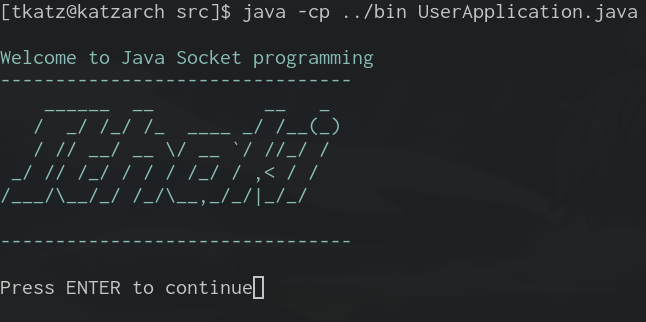
\includegraphics[height=.3\textheight, width=\textwidth]{assets/ui_welcome.png}
	\caption{Welcome screen!} 
    \label{fig:ui}
\end{figure}


Στη συνέχεια παρουσιάζεται μια λίστα με αριθμούς, όπου κάθε αριθμός αντιστοιχίζεται στην εκάστοτε εφαρμογή. Σε περίπτωση που η είσοδος είναι κάτι διαφορετικό απο αυτούς τους αριθμούς τότε ξανά ζητείται απο τον χρήστη να πατήσει έναν απο τους διαθέσιμους. Σε εφαρμογές όπως Ithakicopter UDP passive και στο autopilot που χρησιμοποιούμε το UDP, άρα χρειαζόμαστε και το ithakicopter.jar, έχουμε blocking σημείο στο οποίο ζητάται απο τον χρήστη να ανοίξει το jar και να πατήσει ENTER για να συνεχίσει η εφαρμογή (όπως κάνουμε δηλαδή και στο welcome σημείο).

\begin{figure}[h!]
\centering
	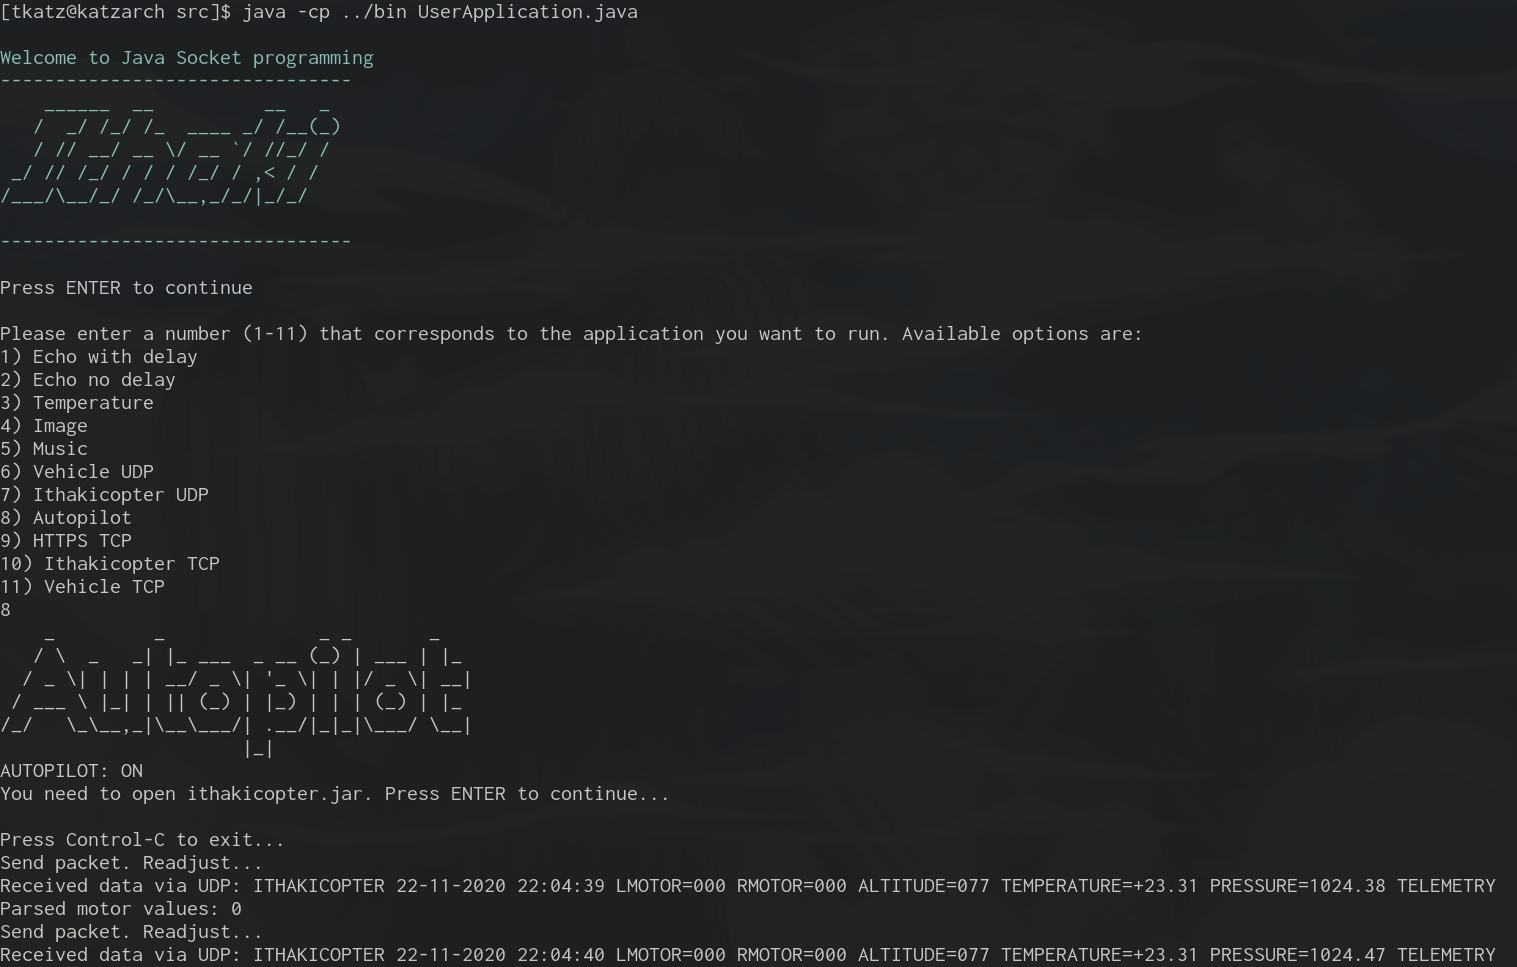
\includegraphics[height=.3\textheight, width=\textwidth]{assets/ui.png}
	\caption{Εκτέλεση προγράμματος σε κέλυφος Bash. Επιλογή Autopilot} 
    \label{fig:ui}
\end{figure}

% \begin{figure}
%      \begin{subfigure}[b]{.5\textwidth}
%          \centering
%          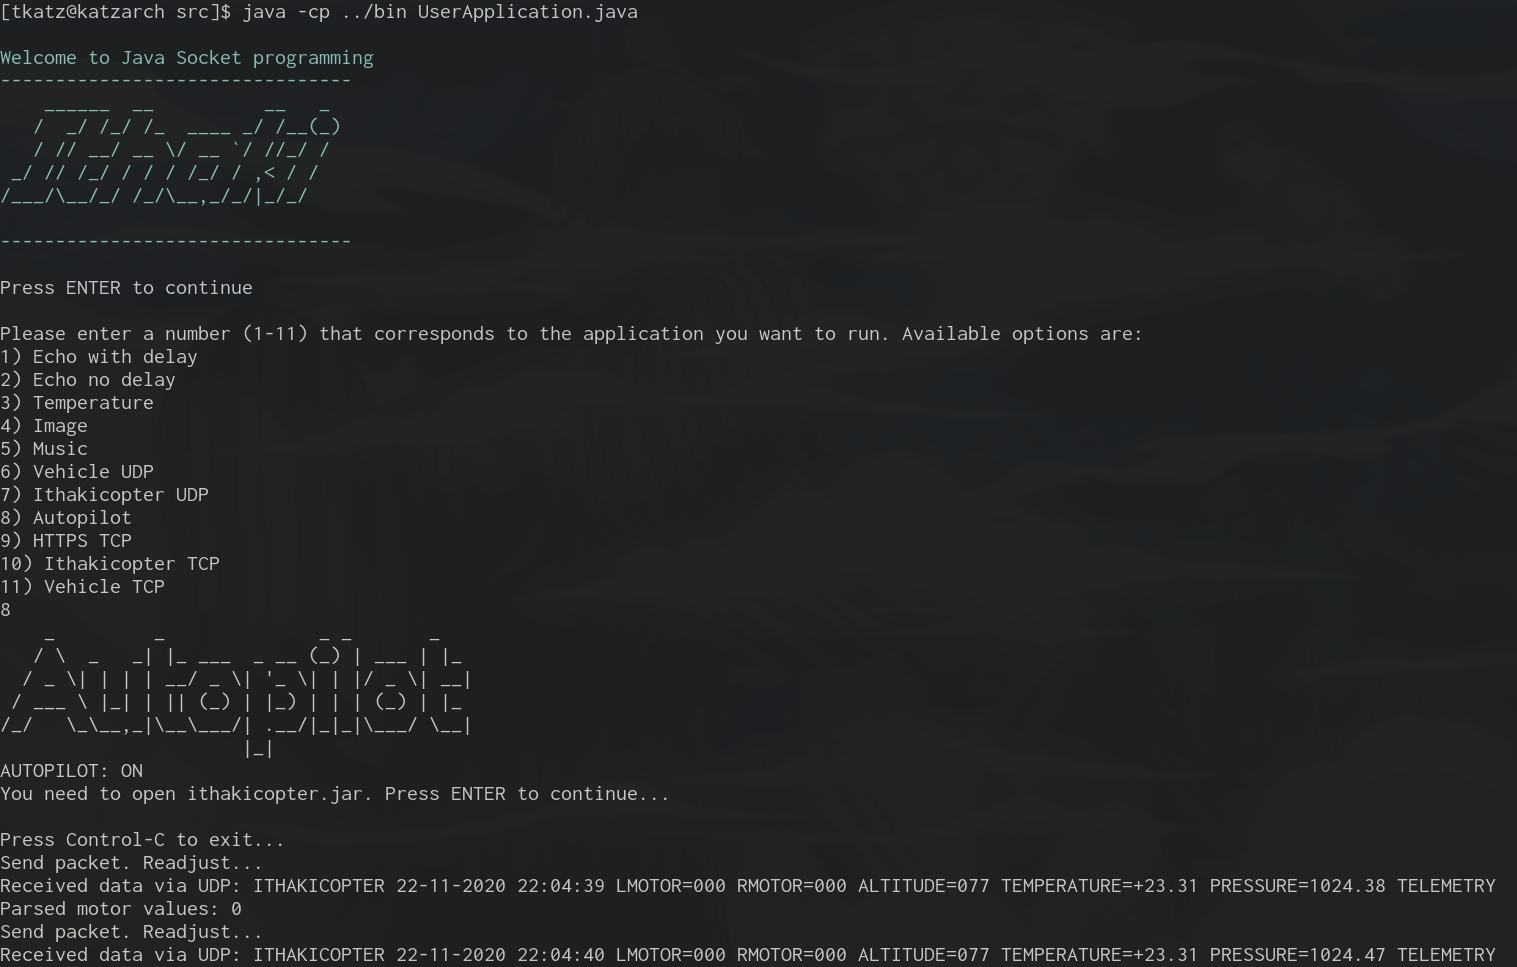
\includegraphics[width=\textwidth]{assets/ui.png}
%          \caption{$y=3sinx$}
%      \end{subfigure}
%      \hfill
%      \begin{subfigure}[b]{.5\textwidth}
%          \centering
%          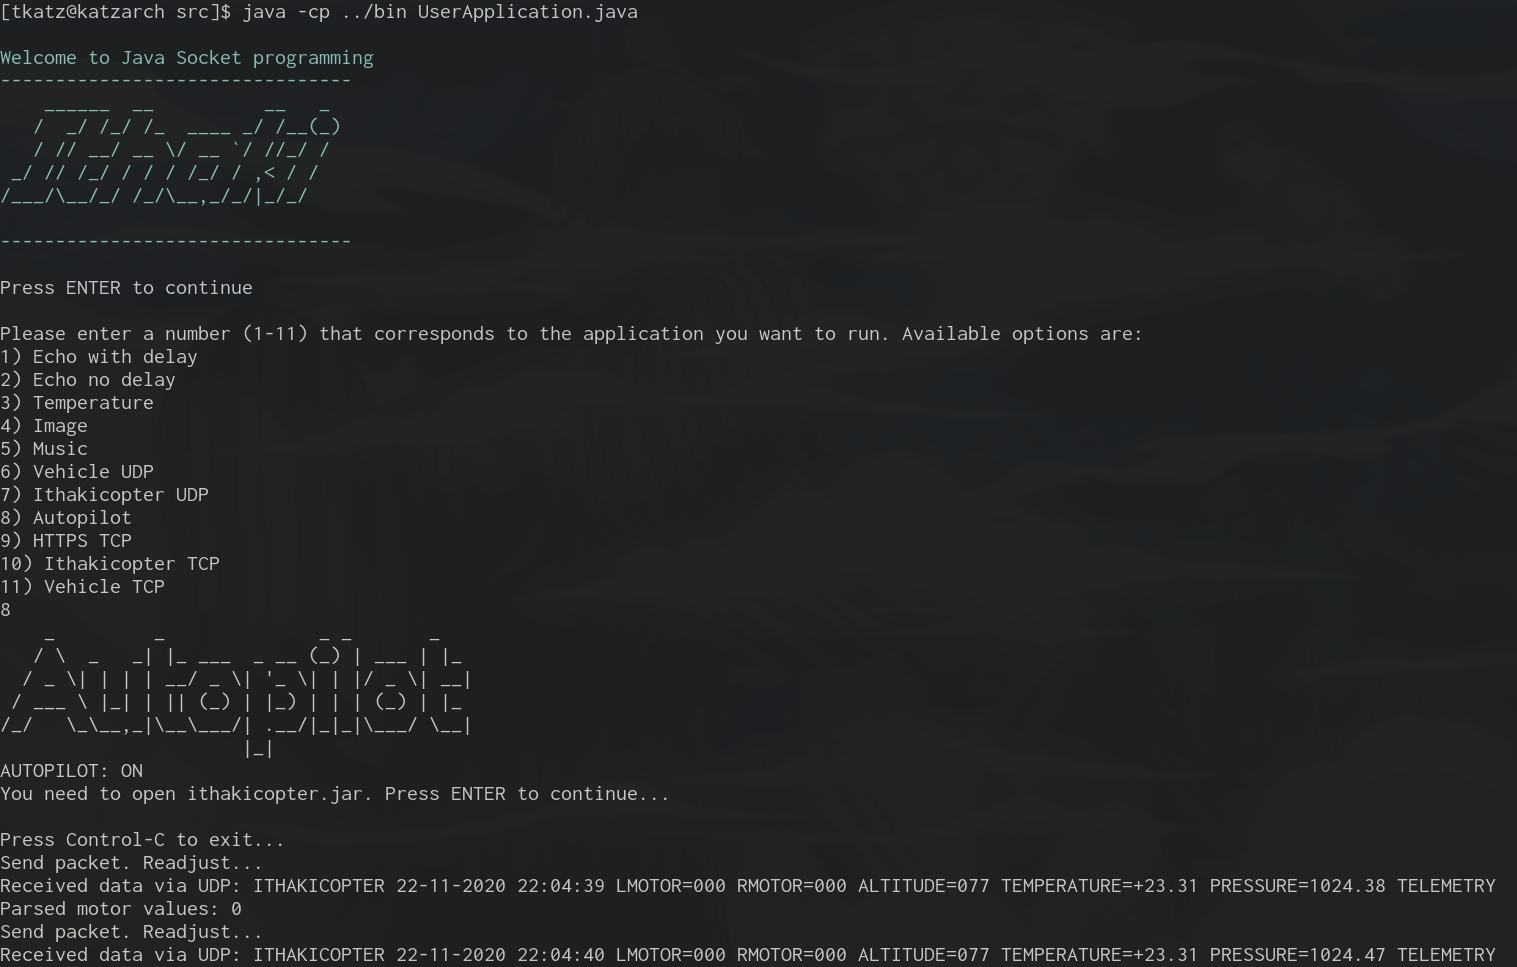
\includegraphics[width=\textwidth]{assets/ui.png}
%          \caption{$y=5/x$}
%      \end{subfigure}
%         \caption{Three simple graphs}
%         \label{fig:three graphs}
% \end{figure}

\pagebreak

\section{UDP}


Τα UDP (User Datagram Protocol) και TCP (Transmission Control Protocol) είναι δύο πολύ βασικά και γνωστά πρωτόκολλα στον χώρο των δικτύων και αφορούν το 4ο επίπεδο, transport layer, του \textbf{OSI (Open Systems Interconnection) communication model}. Συγκεκριμένα για το UDP, είναι ένα πρωτόκολλο το οποίο θέτει ως προτεραιότητα την ταχύτητα της επικοινωνίας παρά την αξιοπιστία\footnote{Για αυτό πολλές φορές το UDP αναφέρεται ως \textbf{Unreliable} Datagram Protocol}. Η δομή του δεν προβλέπει την επιβεβαίωση των πακέτων αποστολής στον επιθυμητό receiver και η αποστολή γίνεται με την λεγόμενη τεχνική \textbf{best effort}. Με λίγα λόγια, ο πομπός στέλνει και ο δέκτης λαμβάνει ό,τι κατάφερε η σύνθετη δομή των δικτύων να μεταφέρει, συμπεριλαμβάνοντας διάφορες πηγές θορύβου. Αυτός ο τρόπος καθίδρυσης επικοινωνίας επιφέρει, απο την άλλη πλευρά, σημαντικά πλεονεκτήματα στην ταχύτητα λήψης πληροφορίας και στον αριθμό των δεδομένων σε σύντομα χρονικά διαστήματα. Για αυτόν τον λόγο εφαρμόζεται συνήθως σε time-sensitive εφαρμογές όπως για παράδειγμα VoIP, audio και συγχρονισμού ώρας, προκειμένου να αποφευχθεί το overhead των handshakes σε υλοποίηση TCP \cite{searchnetworking, wiki_udp}.

Οι θύρες ή αλλιώς τα λεγόμενα \textbf{ports}, μια επίσης πολύ συνηθισμένη και βασική έννοια των δικτύων, στα πλαίσια του 4ου επιπέδου, είναι ένας \textbf{λογικός} (σε αντίθεση με τα physical ports) τρόπος καταμοιρασμού των εργασιών που υλοποιεί ενας υπολογιστικός κόμβος σε ένα δίκτυο. 'Ενας server μπορεί να είναι υπεύθυνος για διάφορα είδη αιτημάτων και υπηρεσιών. Προκειμένου να διαχωρίσουμε τι ζητάει ένας χρήστης απο ένα server υπάρχει μια σύμβαση όσον αφορά τον αριθμό του port που αντιστοιχεί σε κάθε εφαρμογή. Η ίδια λογική των ports εφαρμόζεται τόσο απο την πλευρά του server όσο και απο την πλευρά του client. Η διαφορά είναι ότι συνήθως ports που σχετίζονται με υπηρεσίες των servers είναι standard/προκαθορισμένα (\textbf{well known ports}) ενώ στην πλευρά του client, το λειτουργικό σύστημα αυθαίρετα αναθέτει αριθμό port. Συνεπώς οι θύρες είναι μια αρκετά σημαντική πληροφορία. Στο πρωτόκολλο UDP εμπεριέχεται στο \textbf{header} των fixed 8 bytes. Πιο συγκεκριμένα ένα UDP πακέτο αποτελείται απο τον header και τα data/δεδομένα. Στον header υπάρχουν "εισαγωγικές" πληροφορίες για το είδος των δεδομένων και τον σκοπό της επικοινωνίας. Αναλυτικότερα αποτελείται απο 4 τμήματα των 2 bytes το καθένα. Αυτά είναι το α) source port, ο αριθμός port δηλαδή του κόμβου του δικτύου που στέλνει πληροφορία/αίτημα, β) destination port, σε ποιον πηγαίνει το πακέτο, γ) length, το μήκος του πακέτου και τέλος δ) το checksum, το οποίο χρησιμοποιείται για λόγους ανίχνευσης σφάλματος στην πληροφορία που προσπαθούμε να μεταδώσουμε \cite{wiki_udp, gfgudp}.


\begin{figure}[h!]
     \begin{subfigure}[b]{0.5\textwidth}
         \centering
         
\includegraphics[height=.28\textheight, width=\textwidth]{assets/meme.jpg}
     \end{subfigure}
     \hfill
     \begin{subfigure}[b]{0.5\textwidth}
         \centering
         
\includegraphics[height=.28\textheight, width=\textwidth]{assets/meme2.jpg}
     \end{subfigure}
     \caption{UDP and TCP in a nutshell}
\end{figure}



\section{Audio streaming protocols}

Γενικότερα το streaming στην εποχή μας είναι πλέον διαδεδομένο και υπάρχουν πολλές πλατφόρμες που προσφέρουν τέτοιες υπηρεσίες. Streaming συνοπτικά είναι η δυνατότητα μεταφοράς και αναπαραγωγής δεδομένων που σχετίζονται με πολυμέσα (εικόνα, video, audio) με δυναμικό τρόπο (real time) χωρίς να χρειάζεται να κατέβει όλη η πληροφορία εξαρχής. Με άλλα λόγια audio streaming, είναι κάτι σαν audio on the go. Για να υπάρχει αυτό το αίσθημα της συνεχόμενης ροής πληροφορίας χωρίς διακοπές και καθυστερήσεις, υπολογιστικά είναι μια αρκετά  δύσκολη διαδικασία  και υπάρχουν αυξημένες απαιτήσεις απο το δίκτυο τόσο απο τον provider όσο και απο τον client (media players, internet access, bandwidth). 

Έννοιες σχετικές με αυτήν την θεματολογία είναι η συμπίεση, η κωδικοποίηση και η αποκωδικοποίηση πληροφορίας. Η ποσότητα πληροφορίας που αφορά τα πολυμέσα είναι ιδιαίτερα μεγάλη και η συμπίεση της επιβάλλεται, έτσι ώστε το streaming να είναι εφικτό τόσο στο κομμάτι της επεξεργασίας όσο και στην αποθήκευση. Η συσκευή κωδικοποίησης και αποκωδικοποίησης ονομάζεται codec.

Τα streaming protocols ανήκουν στα application, presentation, session επίπεδα του OSI model, δηλαδή πάνω απο το transport layer (UDP και TCP). Μια σύνοψη για streaming protocols τα οποία μπορούν να χρησιμοποιηθούν και για audio είναι η ακόλουθη \cite{wowza, stackexchange_audio, wowza_rtsp}.

\subsection{HTTP}

HTTP είναι ένα πρωτόκολλο το οποίο κάθεται στο application layer και μπορεί να χρησιμοποιηθεί εκτός των άλλων και για streaming. Είναι μια αρκετή βολική λύση μιας και οι web servers μπορεί να το υποστηρίξουν χωρίς να υπάρχει ανάγκη κάποιου dedicated server για streaming, όπως στην περίπτωση του RTMP πρωτοκόλλου. 

Πρωτόκολλα βασισμένα σε HTTP είναι το \textbf{HTL} (HTTP Live Streaming) το οποίο αναπτύχθηκε απο την Apple και θεωρείται ίσως η πιο δημοφιλής επιλογή για streaming \cite{wiki_hls}, MPEG-DASH (για video), Microsoft Smooth Streaming και το Adobe HDS. Μάλιστα το HLS, το οποίο είναι TCP based, παρέχει την δυνατότητα στους χρήστες να προσαρμόζουν το bitrate στην καλύτερη δυνατή κατάσταση της σύνδεσης τους.

\subsection{SHOUTcast και Icecast}

SHOUTcast και Icecast είναι δύο ακόμη HTTP based πρωτόκολλα για streaming audio data και ιδιαίτερα γνωστά για internet radio. To πρώτο proprietary ενώ το δεύτερο free and open source και μια πολύ καλή εναλλακτική λύση.

\subsection{WebRTC}

Web Real Time Communication είναι ένα σύνολο απο standards το οποίο αφορά peer to peer αρχιτεκτονική για μεταφορά πληροφορίας δίχως να χρειάζονται centralized servers. Είναι UDP based και το μόνο που χρειάζεται για να λειτουργήσει είναι ένας browser \cite{webrtc}.

\subsection{RTMP}

RTMP (Real Time Messaging Protocol) είναι ένα παραδοσιακό πρωτόκολλο το οποίο υποστηριζόταν απο την Adobe. Ωστόσο θεωρείται edged out έπειτα την παύση λειτουργίας του Adobe Flash Player και δεν είναι συνηθισμένη επιλογή πλέον. Αν και μεγάλα ονόματα της βιομηχανίας όπως Facebook συνεχίζουν να χρησιμοποιούν αυτό το πρωτόκολλο \cite{streamingmedia}


\clearpage

\bibliographystyle{plain}
\bibliography{bib/bib.bib}

\end{document}
